% \iffalse
\let\negmedspace\undefined
\let\negthickspace\undefined
\documentclass[journal,12pt,twocolumn]{IEEEtran}
\usepackage{cite}
\usepackage{amsmath,amssymb,amsfonts,amsthm}
\usepackage{algorithmic}
\usepackage{graphicx}
\usepackage{textcomp}
\usepackage{xcolor}
\usepackage{txfonts}
\usepackage{listings}
\usepackage{enumitem}
\usepackage{mathtools}
\usepackage{gensymb}
\usepackage{comment}
\usepackage[breaklinks=true]{hyperref}
\usepackage{tkz-euclide} 
\usepackage{listings}
\usepackage{gvv}  
\usepackage{tikz}
\usepackage{circuitikz} 
\usepackage{caption}
\def\inputGnumericTable{}              
\usepackage[latin1]{inputenc}          
\usepackage{color}                    
\usepackage{array}                     
\usepackage{longtable}                 
\usepackage{calc}                     \usepackage{multirow}                  
\usepackage{hhline}                    
\usepackage{ifthen}                    
\usepackage{lscape}
\usepackage{amsmath}
\newtheorem{theorem}{Theorem}[section]
\newtheorem{problem}{Problem}
\newtheorem{proposition}{Proposition}[section]
\newtheorem{lemma}{Lemma}[section]
\newtheorem{corollary}[theorem]{Corollary}
\newtheorem{example}{Example}[section]
\newtheorem{definition}[problem]{Definition}
\newcommand{\BEQA}{\begin{eqnarray}}
\newcommand{\EEQA}{\end{eqnarray}}
\newcommand{\define}{\stackrel{\triangle}{=}}
\theoremstyle{remark}
\newtheorem{rem}{Remark}

\begin{document}

\bibliographystyle{IEEEtran}
\vspace{3cm}

\title{Audio Filtering}
\author{EE23BTECH11009 - AROSHISH PRADHAN$^{*}$% <-this % stops a space
}
\maketitle
\newpage
\bigskip

\begin{table}[!h]
    \centering
    \begin{tabular}{|c|c|}
\hline
  \textbf{Symbol} & \textbf{Description} \\
\hline
   $x(n)$  & Input Audio Signal \\
\hline
   $y(n)$  & Output Audio Signal \\
\hline
   $H(\omega)$ & Transfer Function \\
\hline
    $h(n)$ & Impulse Response\\
\hline
\end{tabular}

    \caption{Parameter Table}
    \label{tab:parameters}
\end{table}

Plot of input audio signal 'music7\_cut.wav' as $x(n)$:
\begin{figure}[!h]
    \centering
    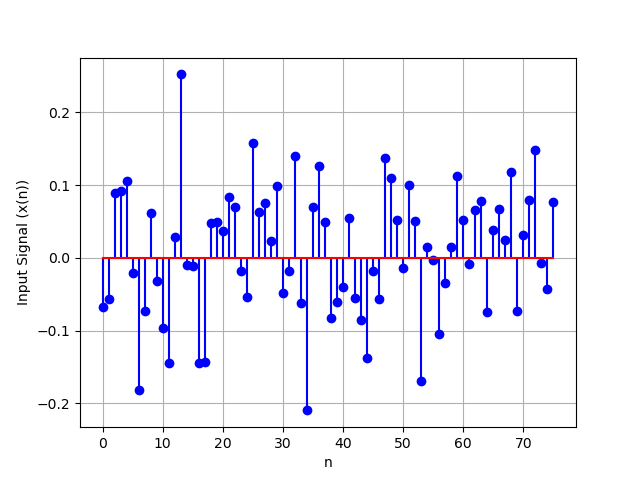
\includegraphics[width = \columnwidth]{figs/x_plot.png}
    \caption{Plot of $x(n)$ vs $n$}
    \label{fig:x_plot}
\end{figure}

$y(n)$ is obtained through the following difference equation:
\begin{align}
    \sum_{m=0}^{M}a(m)y(n-m) = \sum_{k=0}^{N}b(k)x(n-k)
\end{align}
Coefficients $a$ and $b$ are calculated in 'audiofilter.py'
\begin{figure}[!h]
    \centering
    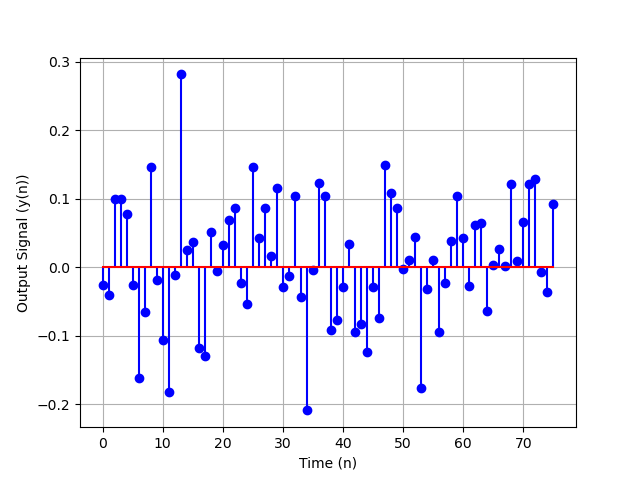
\includegraphics[width = \columnwidth]{figs/y_plot.png}
    \caption{Plot of $y(n)$ vs $n$}
    \label{fig:y_plot}
\end{figure}

Plot of y(n) is as shown in \figref{fig:y_plot}.
\begin{align}
    x(n) &\system{F} X(\omega)\\
    y(n) &\system{F} Y(\omega)\\
    \implies H(\omega) &= \frac{Y(\omega)}{X(\omega)} 
\end{align}
Plot of $H(\omega)$ is shown in \figref{fig:H_plot}

\begin{figure}[!h]
    \centering
    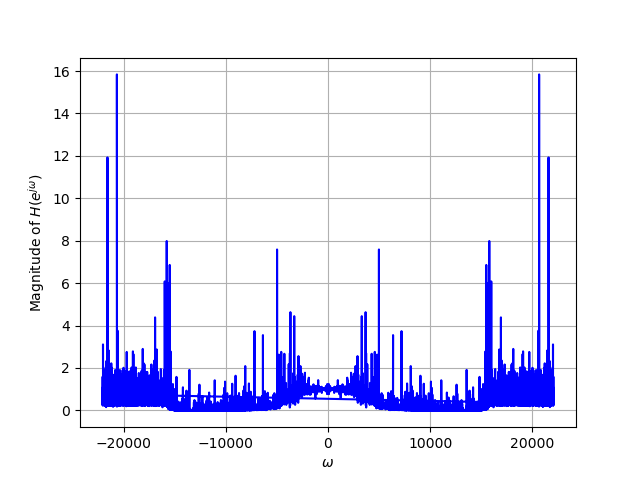
\includegraphics[width = \columnwidth]{figs/H_plot.png}
    \caption{Plot of $H(\omega)$ vs $\omega$}
    \label{fig:H_plot}
\end{figure}

\newpage
Impulse Response ($h(n)$) is calculated by taking the Inverse Fourier Transform of $H(\omega)$.
Plot of $h(n)$ vs $n$ is shown in \figref{fig:h_n_plot}
\begin{figure}[!h]
    \centering
    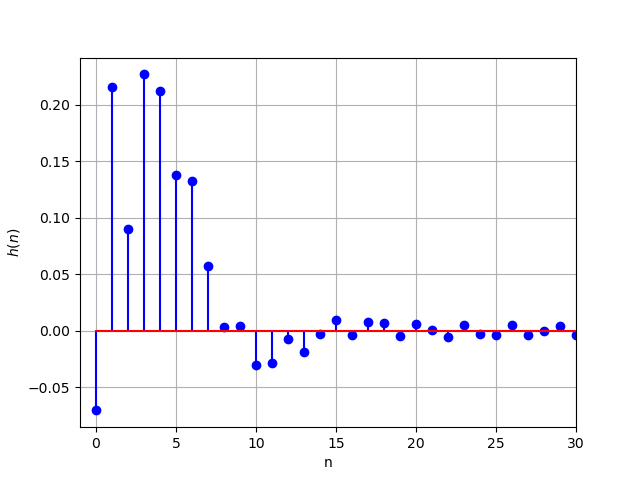
\includegraphics[width = \columnwidth]{figs/h_n.png}
    \caption{Plot of $h(n)$ vs $n$}
    \label{fig:h_n_plot}
\end{figure}

\end{document}
